\section{Progettazione della rete}
\hspace{24pt}Per la realizzazione di questa rete è necessario che i server e le postazioni e le stampanti della reception abbiano una scheda di rete di 1 GBit/s. Le postazioni e le stampanti degli uffici, invece, hanno bisogno di una scheda di rete wireless, in particolare si andrà ad utilizzare una scheda \mintinline{batch}{WMP300N}, la quale dota il computer di un'interfaccia di rete che lavora a 2.4GHz. Per sfruttare al massimo le schede di rete è necessario che anche gli switch abbiano porte da 1 GBit/s e che l'AP lavori a 2.4GHz. Si ha infine bisogno dei cavi, in questo caso UTP\footnote{Unshielded Twisted Pair} di 1 GBit/s di categoria 6. Tenendo sempre in considerazione la scalabilità e la flessibilità della rete, si ha quindi bisogno dei seguenti dispositivi di rete:\\
\begin{itemize}
	\item 4 switch: uno da 4 porte per la stanza server, due da 8 porte per il centro stella e la reception.
	\item 1 AP, per la connessione wireless dei due uffici.
	\item 1 router, per la connessione a Internet
	\item 10 cavi UTP: 3 per le connessioni computer - switch, 1 per la connessione stampante - switch, 2 per le connessioni server - switch, 2 per le connessioni switch - centro stella, 1 per la connessione AP - centro stella e uno per la connessione centro stella - router.
\end{itemize}
Di seguito la rappresentazione grafica della rete.
\vspace{30pt}
\begin{figure}[!h]
	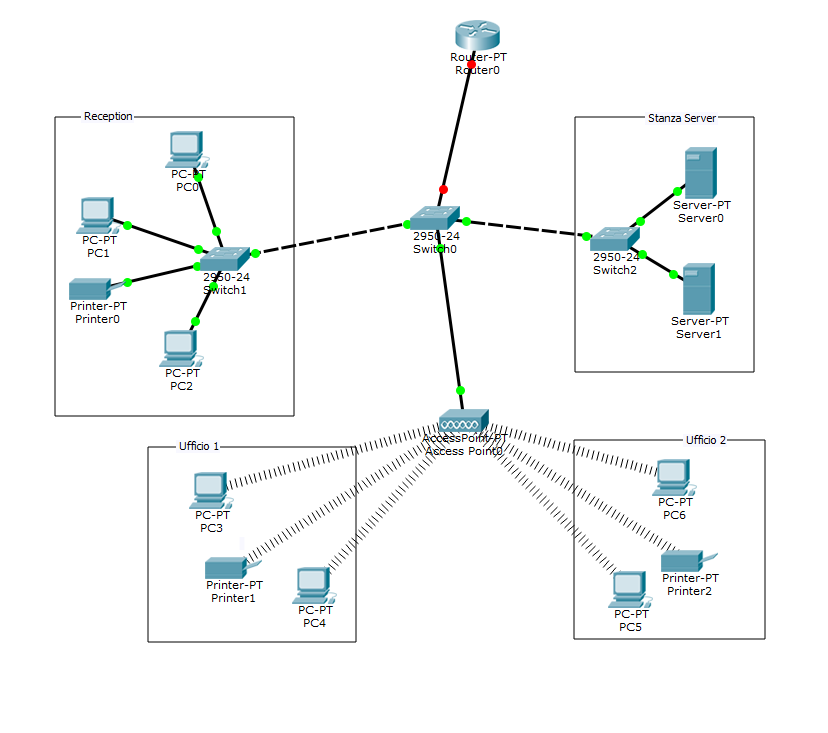
\includegraphics[scale=0.81]{progettazione_rete}
	\label{fig:pr1}
\end{figure}